%
% filter.tex -- Filterung des Trägers
%
% (c) 2018 Prof Dr Andreas Müller, Hochschule Rapperswil
%
\documentclass[tikz,12pt]{standalone}
\usepackage{times}
\usepackage{amsmath}
\usepackage{txfonts}
\usepackage[utf8]{inputenc}
\usepackage{graphics}
\usepackage{color}
\usepackage{pifont}
\usetikzlibrary{arrows,intersections,math,calc}
\begin{document}

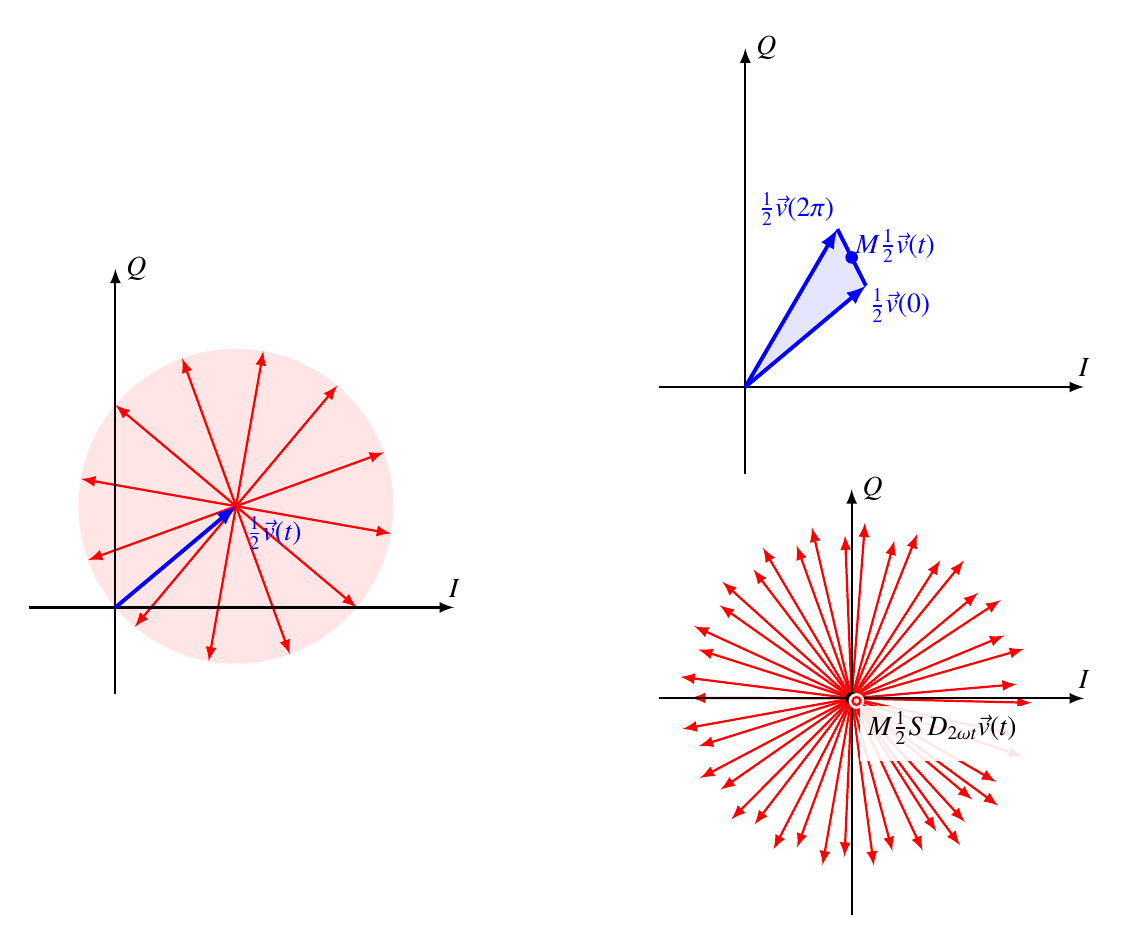
\begin{tikzpicture}[>=latex,thick]

\def\a{40}
\def\r{4}

\begin{scope}[xshift=-4cm]

\fill[color=red!10] ({0.5*\r*cos(\a)},{0.5*\r*sin(\a)}) circle[radius={0.5*\r}];

\foreach \p in {20,50,...,360}{
	\draw[->,color=red] ({0.5*\r*cos(\a)},{0.5*\r*sin(\a)})
		--
	({0.5*\r*cos(\a)+0.5*\r*cos(\p)},{0.5*\r*sin(\a)+0.5*\r*sin(\p)});
}

\draw[->] (-1.1,0)--(4.3,0) coordinate[label={$I$}];
\draw[->] (0,-1.1)--(0,4.3) coordinate[label={right:$Q$}];

\draw[->,line width=1.4pt,color=blue]
	(0,0)--({0.5*\r*cos(\a)},{0.5*\r*sin(\a)});

\node[color=blue] at ({0.5*\r*cos(\a)},{0.5*\r*sin(\a)}) [below right]
	{$\frac12\vec{v}(t)$};

\end{scope}

\pgfmathparse{0.5*\r*cos(\a)}
\xdef\X{\pgfmathresult}
\pgfmathparse{0.5*\r*sin(\a)}
\xdef\Y{\pgfmathresult}

\def\vX{-0.001}
\def\vY{0.002}

\begin{scope}[xshift=4cm,yshift=2.8cm]

\draw[->] (-1.1,0)--(4.3,0) coordinate[label={$I$}];
\draw[->] (0,-1.1)--(0,4.3) coordinate[label={right:$Q$}];

\fill[color=blue!10]
	(0,0)
	--
	({0.5*\r*cos(\a)},{0.5*\r*sin(\a)})
	--
	({0.5*\r*cos(\a)+\vX*360},{0.5*\r*sin(\a)+\vY*360})
	--cycle;

\draw[color=blue,line width=1.4pt] plot[domain=0:360,samples=100]
	({0.5*\r*cos(\a)+\vX*\x},{0.5*\r*sin(\a)+\vY*\x});

\fill[color=blue] 
	({0.5*\r*cos(\a)+\vX*180},{0.5*\r*sin(\a)+\vY*180})
	circle[radius=0.08];
\node[color=blue] at ({0.5*\r*cos(\a)+\vX*180-0.1},{0.5*\r*sin(\a)+\vY*180-0.2})
	[above right] {$M\frac12\vec{v}(t)$};

\draw[->,line width=1.4pt,color=blue]
	(0,0)--({0.5*\r*cos(\a)},{0.5*\r*sin(\a)});
\draw[->,line width=1.4pt,color=blue]
	(0,0)--({0.5*\r*cos(\a)+\vX*360},{0.5*\r*sin(\a)+\vY*360});

\node[color=blue,line width=1.4pt]
	at ({0.5*\r*cos(\a)-0.1},{0.5*\r*sin(\a)+0.1})
	[below right] {$\frac12\vec{v}(0)$};
\node[color=blue,line width=1.4pt]
	at ({0.5*\r*cos(\a)+\vX*360+0.1},{0.5*\r*sin(\a)+\vY*360-0.1})
	[above left] {$\frac12\vec{v}(2\pi)$};

\end{scope}

\pgfmathparse{\X+\vX*180}
\xdef\XX{\pgfmathresult}
\pgfmathparse{\Y+\vY*180}
\xdef\YY{\pgfmathresult}

% XXX why would we show this?
%\node at (0,0) [above] {$X=\XX$};
%\node at (0,0) [below] {$Y=\YY$};

%\begin{scope}[xshift=4cm,yshift=-2.8cm]
\begin{scope}[xshift=5.3508cm,yshift=-1.15461cm]

\foreach \p in {0,8.5,...,359}{
	\draw[->,color=red]
		(0,0)
		--
		({2*((\X+\vX*\p)*cos(\p)-(\Y+\vY*\p)*sin(\p))*cos(\p)-\X-\vX*\p},{-2*((\X+\vX*\p)*cos(\p)-(\Y+\vY*\p)*sin(\p))*sin(\p)-\Y-\vY*\p});
	;
}

\draw[->] (-2.4508,0)--(2.9492,0) coordinate[label={$I$}];
\draw[->] (0,-2.74539)--(0,2.65461) coordinate[label={right:$Q$}];

\xdef\Sx{0}
\xdef\Sy{0}

\foreach \p in {0,1,...,360}{
	\pgfmathparse{\Sx+2*((\X+\vX*\p)*cos(\p)-(\Y+\vY*\p)*sin(\p))*cos(\p)-\X-\vX*\p}
	\xdef\Sx{\pgfmathresult}
	\pgfmathparse{\Sy-2*((\X+\vX*\p)*cos(\p)-(\Y+\vY*\p)*sin(\p))*sin(\p)-\Y-\vY*\p}
	\xdef\Sy{\pgfmathresult}
}
\pgfmathparse{\Sx/361}
\xdef\Sx{\pgfmathresult}
\pgfmathparse{\Sy/361}
\xdef\Sy{\pgfmathresult}

\fill (0,0) circle[radius=0.08];
\fill[color=red!10] ({\Sx},{\Sy}) circle[radius=0.10];
\draw[color=red] ({\Sx},{\Sy}) circle[radius=0.05];

\fill[color=white,opacity=0.9]
	(0.1,-0.1) rectangle (2.3,-0.8);
\node at ({\Sx},{\Sy}) [below right] {$M\frac12SD_{2\omega t}\vec{v}(t)$};

\end{scope}


\end{tikzpicture}

\end{document}

